\documentclass[a4paper, 12pt]{article}
\usepackage[portuges]{babel}
\usepackage[utf8]{inputenc}
\usepackage{amsmath}
\usepackage{indentfirst}
\usepackage{graphicx}
\usepackage{placeins}
\usepackage{multicol,lipsum}
\usepackage{indentfirst}
\usepackage[nottoc,notlot,notlof]{tocbibind}
\setlength{\parindent}{0.6cm}
\newcommand\tab[1][0.6cm]{\hspace*{#1}}

    
    
\begin{document}
\sloppy
\begin{titlepage}
  \begin{center}
      \Huge{Universidade Federal de Pernambuco}\\
      \large{Deep Logic Networks: Inserting and Extracting
Knowledge From Deep Belief Networks}\\ 
      \vspace{15pt}
      \vspace{95pt}
      \textbf{\LARGE{Relatório}}\\
      \vspace{3,5cm}
  \end{center}

  \begin{flushleft}
      \begin{tabbing}
                  José Nilton\\
                  Italo Paulino\\
                  Mateus Gonçalves\\ 
                  Wallace Soares\\
      \end{tabbing}
  \end{flushleft}
  \vspace{1cm}

  \begin{center}
      \vspace{\fill}
      Junho - 2018\\
  \end{center}
\end{titlepage}
\newpage
\tableofcontents
\thispagestyle{empty}
\newpage
\pagenumbering{arabic}
\section{Introdução}
O uso de redes \textit{deep} para resolução de problemas complexos envolvendo \textit{Big Data} vem sendo cada vez mais comum nas ultimas décadas. Entretanto, compreender o treinamento deste tipo de rede não é trivial. Áreas como a \textit{neural-symbolic computing} estudam em como o conhecimento pode ser inserido e extraído de redes neurais \textit{deep} \cite{Tran}, \cite{garbook}, \cite{garConf}. Através da inserção de conhecimento Tran e Garcez \cite{Tran} mostraram que é possível economizar tempo de processamento na aprendizagem, pois tal inserção já será uma alternativa a fase de pré-treinamento.
Tran e Garcez também mostram que a extração de conhecimento é um importante fator que pode ser adicionado a este tipo de rede. Por dois motivos: compreensão e a própria inserção de conhecimento. Compreensão pois podemos entender como está a fase de treinamento nas camadas intermediárias. Inserção pois uma vez em que sabemos como cada unidade aprendeu a reproduzir o padrão de entrada podemos modificar o conhecimento da rede para obter um menor gasto de processamento na fase de treinamento.

O artigo em análise propõe um método de inserção e extração de conhecimento em \textit{Deep Belief Networks} (DBNs) através das regras de confidência propostas por Tran e Garcez. DBNs são definidas como n-Restricted Boltzman Machines - (RBMs) empilhadas de forma que a camada de escondida de uma RBM seja a camada visivel da próxima como mostra a figura abaixo. Exploramos os conceitos de RBMs, DBNs e regras de confidência nas seções 2.1, 2.2 e 2.3 respectivamente.

\begin{figure}[h]
 \centering
 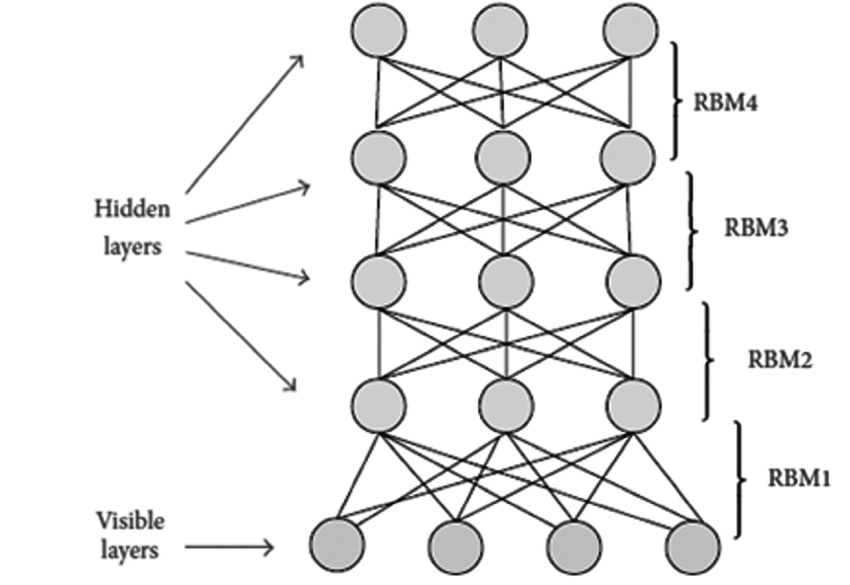
\includegraphics[scale=0.3]{Graphical-Representation-of-a-Deep-Belief-Network.png}
 \caption{Representação gráfica de \textit{Deep Belief Networks}.\cite{imagem1}}
\end{figure}

\section{Conceitos Básicos}
\subsection{Restricted Boltzmann Machines}
RBMs constituem-se por neurônios ligados por grafos bidirecionais que conectam a camada visível à camada escondida. Essa rede é considerada restrita porque não há conexão entre unidades da mesma camada, como nas máquinas de Boltzmann originais. O objetivo desta rede é aproximar ao máximo o resultado da camada escondida com o que esta sendo apresentado na entrada. Através da apresentação do padrão de entrada na camada visivel, RBMs criam padrões numéricos na camada escondida que relacionam diretamente os pesos das arestas com as funções de ativação das camadas visível e escondida. 
\begin{figure}[h]
 \centering
 \includegraphics[scale=0.4]{Restricted-boltzmann-machine_svg.png}
 \caption{Representação gráfica de \textit{Restricted Boltzmann Machines}.\cite{RBM}}
\end{figure}

A partir dos padrões numéricos, a camada escondida tenta reconstruir na camada visível o que foi apresentado como entrada. Este processo é repetido até que a RBMs produza com maior acurácia o padrão de entrada. Apesar desta característica de não supervisionada de detectar padrões, RBMs podem ser utilizadas tanto para aprendizado supervisionado como não-supervisionado. Como dito por \cite{overviewRBM}, RBMs são modelos baseados em energia, isto é para cada estado que a RBM possuir uma energia será associada e assim um probalidade da rede estar representando o padrão de entrada.

\subsection{Deep Beliefs Networks}
DBNs são essencialmente várias RBMs empilhadas em que a camada escondida de uma RBM será a camada visível da próxima, e assim sucessivamente como mostrado na figura 1. Ao contrário das \textit{Convolutional Neural Networks}(CNNs) que precisam dados previamente categorizados para o treinamento, DBNs utilizam as RBMs para reproduzir todo o padrão de entrada camada por camada. Como proposto por Hinton\cite{Hinton} o primeiro passo para o treinamento de uma DBN é usar o algoritmo \textit{contrastive divergence}(CD) para reproduzir na primeira camada o padrão de entrada. O treinamento so passará para a segunda camanda da DBNs após a primeira RBM atingir o máximo valor de energia. Após este passo, a camada escondida da primeira RBM será utilizada como entrada na segunda RBM. Este processo é repetido até que a ultima camada finalize seu treinamento. Entretanto, após a ultima camada finalizar seu treinamento ainda não se sabe como comparar a saida da DBN com dados reais. Para isso utiliza-se algoritmos de aprendizado supervisionado que categoriza a saida da DBNs, identificando os dados com o conjunto de dados utilizado. A vantagem dessa abordagem é de que DBNs necessitam de conjuntos de dados menores para classificação.

\subsection{Regras de Confidência}
Como definido em \cite{Tran}, regras de confidência são formulas bicondicionais(se, somente se) como indicado abaixo:

\begin{equation}
c : h \leftrightarrow x_1 \wedge ... \wedge x_n
\qquad \text{Regra de Confidência}
\end{equation}

Onde $h$ é uma proposição atomica e cada $x_i$ é um literal(uma proposição atômica ou sua negação), classificadas por um valor real $c$ chamado de valor de confidência. As regras de confidência serão utilizadas tanto na extração, como na inserção de conhecimento. Elas guiarão a rede dizendo quais regras devem ser utilizadas para inserção de conhecimento.
	
\section{Módulos}

Esta seção aborda os principais componentes da implementação que são a inferência, a extração e inserção de regras de confidência.
\subsection{Inferência}
As regras de confidência também podem ser classificadas por hierarquias\cite{Tran}. Isto é, utilizar uma regra base que possua todos os valores de confidência da entrada para inferir um sub-conjunto de regras que possuem valores de confidencia distintos. Assim é possível encontrar um sub-conjunto de regras do qual podemos extrair uma regra que possui maior relação com o que está sendo aprensentado na camada visível, e assim relacionando-a a uma unidade da camada escondida. Estes valores, que devem posteriormente a inferência serem normalizados, são apresentados como entrada à segunda camada da hierarquia que irá obter outro sub-conjunto de regras com outros valores de confidência. A partir destas inferências é possível encontrar sub-conjuntos de regras de confidência que podem representar padrões de entrada nas camdas visíveis das RBMs. Normalização se faz necessária porque é preciso manter uma equivalência entre as regras da unidades da RBM.
\subsection{Extração}
O artigo\cite{Tran} propõe extração de regras de uma RBM treinada da seguinte forma: para cada unidade $j$, a regra de confidência segue o modelo abaixo.

\begin{equation}
	c_j : h_j \leftrightarrow \bigwedge_{\forall t \in T} x_t \wedge \bigwedge_{\forall k \in K} x_k
\end{equation}

Em que $x_t$ e $x_k$ representam literais positivos e negativos, respectivamente. A objetivo é através do algoritmo de extração buscar literais positivos e negativos e valores de confidência que minimizem a perda de informação, de acordo com a equação:

\begin{equation}
	I_{loss} = \sum_{ij}||w_{ij} - c_js_{ij} ||^2
\end{equation}

em que $c_j$ é o valor de confidência da regra $j$ correspondente a unidade $j$ de uma unidade escondida\cite{Tran}. $s_{ij}$ sera 1 caso o literal $x_t$ aparecer na regra j; -1 caso o literal $x_k$ aparecer na regra j; 0 caso contrário. Após algumas operações aritméticas detalhadas melhor no artigo, \cite{Tran} chega a conclusão que o literal que possuir um valor de peso abs($w_{ij}$) $\leq$ $c_j/2$ não deve aparecer na regra $j$. Sendo assim somente entradas que possuirem \textit{relevância} para a regra $j$ estarão presentes na mesma.

Seguindo a abordagem de expansão através de várias RBMs empilhadas, podemos aplicar o algoritmo de inferência\cite{Tran} repetidas vezes para expandir a extração para DBNs.

\subsection{Inserção}

Como discutido anteriormente conhecimento hierarquizado, que tem como base a \textit{modus ponens}, associado a valores de cofidência oferece uma representação simbolica para a DBN\cite{Tran}. Dado um conjunto de regras de confidência obtidas na extração podemos atualizar as conexões entre as camadas da DBN como sendo os valores de confidência de cada, respectiva, unidade escondida. Por exemplo: 

\begin{equation}
	K^{(1)} = {c_1 : y_1 \leftrightarrow x_1 \wedge \neg x_2; c_2 : y_2 \leftrightarrow x_2 \wedge x_3;c_3 : y_3 \leftrightarrow \neg x_3 \wedge  x_4 }
\end{equation}
\begin{equation}
K^{(2)} = {c_4 : z_1 \leftrightarrow \neg y_1 \wedge y_2; c_5 : z_2 \leftrightarrow y_3}
\end{equation}
\begin{equation}
K^{(3)} = {c_6 : t_1 \leftrightarrow z_1 \wedge z_2}
\end{equation}

\begin{equation}
	c_1 : y_1 \leftrightarrow x_1 \wedge \neg x_2
\end{equation}

Se a extração de conhecimento obter a regra $c_1 : y_1 \leftrightarrow x_1 \wedge \neg x_2$ acima, uma unidade $y_1$ será adicionada à camada escondida da primeira RBM e com os pesos $w_{11}$ = $c_1$, $w_{21}$ = $-c_1$. Este processo é repetido para todas as regras de $K^{(1)}$ e um peso de retorno das camadas escondidas é iniciado randomicamente. Com isso o artigo mostra que é possível implementar conhecimento à DBN. A partir deste conhecimento o algoritmo \textit{contrastive divergence} é novamente utlizado para treinar a rede obtendo uma melhor acurácia na DBN.

\section{Metodologia de comparação dos resultados}
\section{Conclusão}

\begin{figure}[ht]
 \centering
 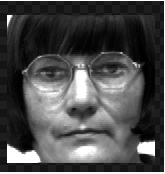
\includegraphics[scale=0.8]{original.png}
 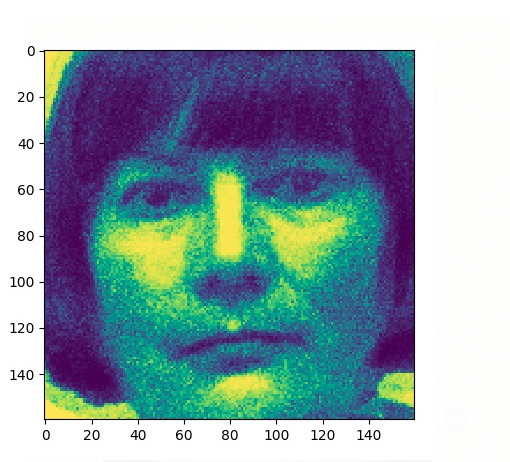
\includegraphics[scale=0.33]{reconstruida.png}
 \caption{Esquerda - Foto original | Direita - Foto reconstruida }
\end{figure}
\bibliographystyle{ieeetr}
\bibliography{sample}
\end{document}
